\subsection{Auto Balancing Bridge} \label{ssec:AutoBalanceBridge}
The auto balancing bridge is build around the principle of feedback, and is often implemented by the use of an operational amplifier, or OP-Amp. The bandwidth is however, somewhat, limited when an OP-Amp is used to implement this technique. To work around this, this principle is sometimes implemented by the use of a null detector, a phase sensitive detector and a phase and amplitude variable generator. This is a rather complex circuitry, and this chapter will only introduce the principle of the auto balancing bridge, and as such treat it like 
an OP-Amp circuit.

\begin{figure}[H]
    \centering
    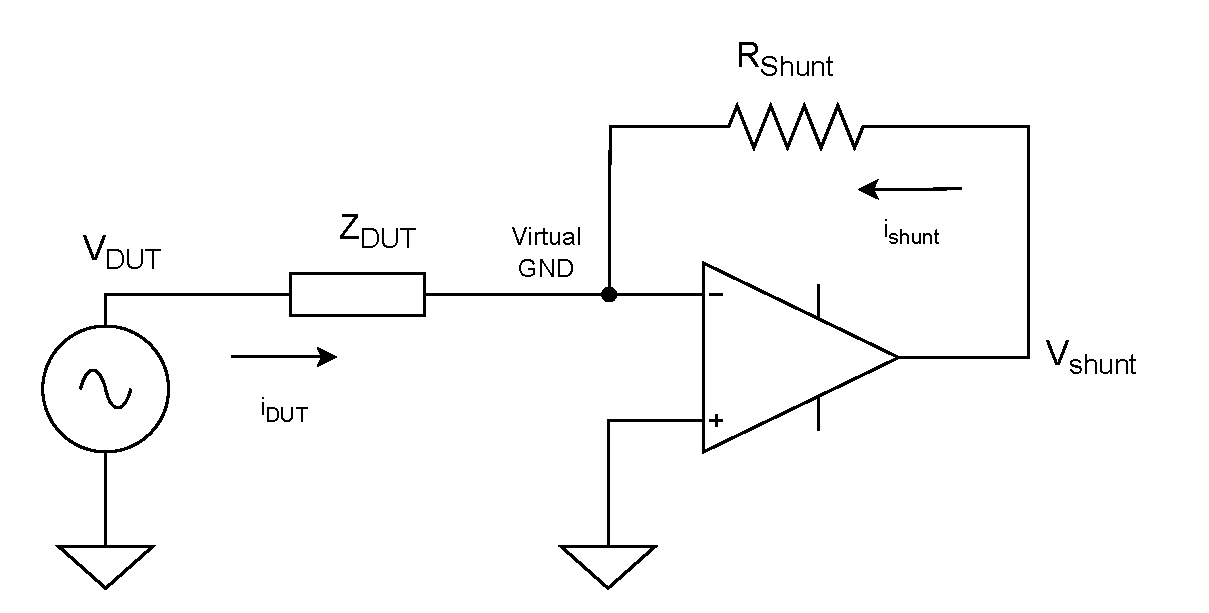
\includegraphics[width=0.75\textwidth]{Sections/4_TechnicalAnalysis/Figures_JFT/AutoBalanceBridge.pdf}
    \caption{The general principle of the auto balancing bridge circuit.}
    \label{fig_4_2_AutoBalanceBridge}
\end{figure}

The principle can be seen on figure \ref{fig_4_2_AutoBalanceBridge}, where the inverting input of the OP-Amp, under ideal assumptions, will be a virtual ground node, thus the voltage across the shunt can simply be measured at the output of the OP-Amp. Likewise the DUT voltage can also be measured at the node named $V_{DUT}$. This has the advantage that no differential measurements needs to be made. Another
advantage of this circuit is that the input capacitance of the circuit that will measure both the DUT and shunt voltage will be connected
to a low impedance source, i.e. the excitation source and the OP-Amp output. This means that these parasitic capacitances will have a minimum effect on the circuit, and as such this topology is among the most precise methods used in impedance analyzers.

It should be noted, that the circuit is configured in an inverting configuration, such that the current measured, as a function of $V_{Shunt}$ will be \SIQ{180}{\degree} phase shifted, compared to the actual DUT current. The circuit is easily analyzed, as an inverting OP-Amp, as seen in equation \ref{eq:4_2_3AutoBalanceBridge1}.
\begin{equation}
    \label{eq:4_2_3AutoBalanceBridge1}
    \begin{split}
        \frac{v_o}{v_i} &= -\frac{R_{Shunt}}{Z_{DUT}}\\
        v_{DUT} &= v_i \qquad v_{Shunt} = v_o \\
        \Rightarrow Z_{DUT} &= -\frac{R_{Shunt}\cdot v_{Shunt}}{v_{DUT}}
    \end{split}
\end{equation}
Equation \ref{eq:4_2_3AutoBalanceBridge1} does however not paint the full picture, as the voltages are complex vectors. Assuming that the phase of the source voltage will not change, equation \ref{eq:4_2_3AutoBalanceBridge1} can be expanded by modeling 
the shunt voltage as a voltage and a phase

\begin{equation}
    \label{eq:4_2_3AutoBalanceBridge2}
    \begin{split}
        Z_{DUT} &= -\frac{R_{Shunt}\cdot v_{Shunt}}{v_{DUT}} \\
        \Rightarrow \vec{Z_{DUT}} &= -\frac{R_{Shunt}\cdot |\vec{v_{Shunt}}|\cdot\e ^{j\theta}}{|\vec{v_{DUT}|}} \\
        \Rightarrow \vec{Z_{DUT}} &= \frac{R_{Shunt}\cdot |\vec{v_{Shunt}}|\cdot\e ^{j\theta}}{|\vec{v_{DUT}|}} \cdot \e ^{-j\pi} \\
        \Rightarrow \vec{Z_{DUT}} &= \frac{R_{Shunt}\cdot |\vec{v_{Shunt}}|\cdot\e ^{j\theta}\cdot \e ^{-j\pi}}{|\vec{v_{DUT}|}}  \\
        \Rightarrow \vec{Z_{DUT}} &= \frac{R_{Shunt}\cdot |\vec{v_{Shunt}}|\cdot\e ^{j(\theta-\pi)}\cdot}{|\vec{v_{DUT}|}}
    \end{split}
\end{equation}

This topology is widely used in precision impedance measurements, especially for frequencies up to a few hundred kHz. At higher frequencies, the OP-Amp gain tends to decrease too much to produce precise results.